\documentclass[conference]{IEEEtran}

% *** CITATION PACKAGES ***
%
%\usepackage{cite}
% cite.sty was written by Donald Arseneau
% V1.6 and later of IEEEtran pre-defines the format of the cite.sty package
% \cite{} output to follow that of IEEE. Loading the cite package will
% result in citation numbers being automatically sorted and properly
% "compressed/ranged". e.g., [1], [9], [2], [7], [5], [6] without using
% cite.sty will become [1], [2], [5]--[7], [9] using cite.sty. cite.sty's
% \cite will automatically add leading space, if needed. Use cite.sty's
% noadjust option (cite.sty V3.8 and later) if you want to turn this off.
% cite.sty is already installed on most LaTeX systems. Be sure and use
% version 4.0 (2003-05-27) and later if using hyperref.sty. cite.sty does
% not currently provide for hyperlinked citations.
% The latest version can be obtained at:
% http://www.ctan.org/tex-archive/macros/latex/contrib/cite/
% The documentation is contained in the cite.sty file itself.

% *** GRAPHICS RELATED PACKAGES ***
%
\ifCLASSINFOpdf
  \usepackage[pdftex]{graphicx}
  % declare the path(s) where your graphic files are
  % \graphicspath{{../pdf/}{../jpeg/}}
  % and their extensions so you won't have to specify these with
  % every instance of \includegraphics
  % \DeclareGraphicsExtensions{.jpg,.jpeg,.png}
\else
  % or other class option (dvipsone, dvipdf, if not using dvips). graphicx
  % will default to the driver specified in the system graphics.cfg if no
  % driver is specified.
  % \usepackage[dvips]{graphicx}
  % declare the path(s) where your graphic files are
  % \graphicspath{{../eps/}}
  % and their extensions so you won't have to specify these with
  % every instance of \includegraphics
  % \DeclareGraphicsExtensions{.eps}
\fi
% graphicx was written by David Carlisle and Sebastian Rahtz. It is
% required if you want graphics, photos, etc. graphicx.sty is already
% installed on most LaTeX systems. The latest version and documentation can
% be obtained at: 
% http://www.ctan.org/tex-archive/macros/latex/required/graphics/
% Another good source of documentation is "Using Imported Graphics in
% LaTeX2e" by Keith Reckdahl which can be found as epslatex.ps or
% epslatex.pdf at: http://www.ctan.org/tex-archive/info/
%
% latex, and pdflatex in dvi mode, support graphics in encapsulated
% postscript (.eps) format. pdflatex in pdf mode supports graphics
% in .pdf, .jpeg, .png and .mps (metapost) formats. Users should ensure
% that all non-photo figures use a vector format (.eps, .pdf, .mps) and
% not a bitmapped formats (.jpeg, .png). IEEE frowns on bitmapped formats
% which can result in "jaggedy"/blurry rendering of lines and letters as
% well as large increases in file sizes.
%
% You can find documentation about the pdfTeX application at:
% http://www.tug.org/applications/pdftex

% *** SPECIALIZED LIST PACKAGES ***
%
%\usepackage{algorithmic}
% algorithmic.sty was written by Peter Williams and Rogerio Brito.
% This package provides an algorithmic environment fo describing algorithms.
% You can use the algorithmic environment in-text or within a figure
% environment to provide for a floating algorithm. Do NOT use the algorithm
% floating environment provided by algorithm.sty (by the same authors) or
% algorithm2e.sty (by Christophe Fiorio) as IEEE does not use dedicated
% algorithm float types and packages that provide these will not provide
% correct IEEE style captions. The latest version and documentation of
% algorithmic.sty can be obtained at:
% http://www.ctan.org/tex-archive/macros/latex/contrib/algorithms/
% There is also a support site at:
% http://algorithms.berlios.de/index.html
% Also of interest may be the (relatively newer and more customizable)
% algorithmicx.sty package by Szasz Janos:
% http://www.ctan.org/tex-archive/macros/latex/contrib/algorithmicx/

% *** ALIGNMENT PACKAGES ***
%
%\usepackage{array}
% Frank Mittelbach's and David Carlisle's array.sty patches and improves
% the standard LaTeX2e array and tabular environments to provide better
% appearance and additional user controls. As the default LaTeX2e table
% generation code is lacking to the point of almost being broken with
% respect to the quality of the end results, all users are strongly
% advised to use an enhanced (at the very least that provided by array.sty)
% set of table tools. array.sty is already installed on most systems. The
% latest version and documentation can be obtained at:
% http://www.ctan.org/tex-archive/macros/latex/required/tools/

%\usepackage{mdwmath}
%\usepackage{mdwtab}
% Also highly recommended is Mark Wooding's extremely powerful MDW tools,
% especially mdwmath.sty and mdwtab.sty which are used to format equations
% and tables, respectively. The MDWtools set is already installed on most
% LaTeX systems. The lastest version and documentation is available at:
% http://www.ctan.org/tex-archive/macros/latex/contrib/mdwtools/

% IEEEtran contains the IEEEeqnarray family of commands that can be used to
% generate multiline equations as well as matrices, tables, etc., of high
% quality.

%\usepackage{eqparbox}
% Also of notable interest is Scott Pakin's eqparbox package for creating
% (automatically sized) equal width boxes - aka "natural width parboxes".
% Available at:
% http://www.ctan.org/tex-archive/macros/latex/contrib/eqparbox/

% *** SUBFIGURE PACKAGES ***
%\usepackage[tight,footnotesize]{subfigure}
% subfigure.sty was written by Steven Douglas Cochran. This package makes it
% easy to put subfigures in your figures. e.g., "Figure 1a and 1b". For IEEE
% work, it is a good idea to load it with the tight package option to reduce
% the amount of white space around the subfigures. subfigure.sty is already
% installed on most LaTeX systems. The latest version and documentation can
% be obtained at:
% http://www.ctan.org/tex-archive/obsolete/macros/latex/contrib/subfigure/
% subfigure.sty has been superceeded by subfig.sty.

%\usepackage[caption=false]{caption}
%\usepackage[font=footnotesize]{subfig}
% subfig.sty, also written by Steven Douglas Cochran, is the modern
% replacement for subfigure.sty. However, subfig.sty requires and
% automatically loads Axel Sommerfeldt's caption.sty which will override
% IEEEtran.cls handling of captions and this will result in nonIEEE style
% figure/table captions. To prevent this problem, be sure and preload
% caption.sty with its "caption=false" package option. This is will preserve
% IEEEtran.cls handing of captions. Version 1.3 (2005/06/28) and later 
% (recommended due to many improvements over 1.2) of subfig.sty supports
% the caption=false option directly:
%\usepackage[caption=false,font=footnotesize]{subfig}
%
% The latest version and documentation can be obtained at:
% http://www.ctan.org/tex-archive/macros/latex/contrib/subfig/
% The latest version and documentation of caption.sty can be obtained at:
% http://www.ctan.org/tex-archive/macros/latex/contrib/caption/

% *** FLOAT PACKAGES ***
%
%\usepackage{fixltx2e}
% fixltx2e, the successor to the earlier fix2col.sty, was written by
% Frank Mittelbach and David Carlisle. This package corrects a few problems
% in the LaTeX2e kernel, the most notable of which is that in current
% LaTeX2e releases, the ordering of single and double column floats is not
% guaranteed to be preserved. Thus, an unpatched LaTeX2e can allow a
% single column figure to be placed prior to an earlier double column
% figure. The latest version and documentation can be found at:
% http://www.ctan.org/tex-archive/macros/latex/base/

%\usepackage{stfloats}
% stfloats.sty was written by Sigitas Tolusis. This package gives LaTeX2e
% the ability to do double column floats at the bottom of the page as well
% as the top. (e.g., "\begin{figure*}[!b]" is not normally possible in
% LaTeX2e). It also provides a command:
%\fnbelowfloat
% to enable the placement of footnotes below bottom floats (the standard
% LaTeX2e kernel puts them above bottom floats). This is an invasive package
% which rewrites many portions of the LaTeX2e float routines. It may not work
% with other packages that modify the LaTeX2e float routines. The latest
% version and documentation can be obtained at:
% http://www.ctan.org/tex-archive/macros/latex/contrib/sttools/
% Documentation is contained in the stfloats.sty comments as well as in the
% presfull.pdf file. Do not use the stfloats baselinefloat ability as IEEE
% does not allow \baselineskip to stretch. Authors submitting work to the
% IEEE should note that IEEE rarely uses double column equations and
% that authors should try to avoid such use. Do not be tempted to use the
% cuted.sty or midfloat.sty packages (also by Sigitas Tolusis) as IEEE does
% not format its papers in such ways.

% *** PDF, URL AND HYPERLINK PACKAGES ***
%
%\usepackage{url}
% url.sty was written by Donald Arseneau. It provides better support for
% handling and breaking URLs. url.sty is already installed on most LaTeX
% systems. The latest version can be obtained at:
% http://www.ctan.org/tex-archive/macros/latex/contrib/misc/
% Read the url.sty source comments for usage information. Basically,
% \url{my_url_here}.

% *** Do not adjust lengths that control margins, column widths, etc. ***
% *** Do not use packages that alter fonts (such as pslatex).         ***
% There should be no need to do such things with IEEEtran.cls V1.6 and later.
% (Unless specifically asked to do so by the journal or conference you plan
% to submit to, of course. )

\usepackage[applemac]{inputenc}
%\usepackage[portuges,brazilian]{babel}
\usepackage[T1]{fontenc}

% correct bad hyphenation here
\hyphenation{op-tical net-works semi-conduc-tor}

\begin{document}
%
% paper title
% can use linebreaks \\ within to get better formatting as desired
\title{Metadata-based Test Framework to Verify External Effects of the Target Classes}
% author names and affiliations
% use a multiple column layout for up to three different
% affiliations
\author{\IEEEauthorblockN{Marcus V. C. Floriano}
\IEEEauthorblockA{Aeronautical Institute of Technology\\
Pra�a Marechal Eduardo Gomes, 50\\
Vl Ac�cias - SJ Campos � SP, Brazil\\
+55 12 39475899\\
Email: marcus.floriano@gmail.com}
\and
\IEEEauthorblockN{Debora A. L. Chama}
\IEEEauthorblockA{Aeronautical Institute of Technology\\
Pra�a Marechal Eduardo Gomes, 50\\
Vl Ac�cias - SJ Campos � SP, Brazil\\
+55 12 39475899\\
Email: deborachama@gmail.com}
\and
\IEEEauthorblockN{Eduardo M. Guerra}
\IEEEauthorblockA{Aeronautical Institute of Technology\\
Pra�a Marechal Eduardo Gomes, 50\\
Vl Ac�cias - SJ Campos � SP, Brazil\\
+55 12 39475899\\
Email: guerraem@gmail.com}}

% conference papers do not typically use \thanks and this command
% is locked out in conference mode. If really needed, such as for
% the acknowledgment of grants, issue a \IEEEoverridecommandlockouts
% after \documentclass

% for over three affiliations, or if they all won't fit within the width
% of the page, use this alternative format:
% 
%\author{\IEEEauthorblockN{Michael Shell\IEEEauthorrefmark{1},
%Homer Simpson\IEEEauthorrefmark{2},
%James Kirk\IEEEauthorrefmark{3}, 
%Montgomery Scott\IEEEauthorrefmark{3} and
%Eldon Tyrell\IEEEauthorrefmark{4}}
%\IEEEauthorblockA{\IEEEauthorrefmark{1}School of Electrical and Computer Engineering\\
%Georgia Institute of Technology,
%Atlanta, Georgia 30332--0250\\ Email: see http://www.michaelshell.org/contact.html}
%\IEEEauthorblockA{\IEEEauthorrefmark{2}Twentieth Century Fox, Springfield, USA\\
%Email: homer@thesimpsons.com}
%\IEEEauthorblockA{\IEEEauthorrefmark{3}Starfleet Academy, San Francisco, California 96678-2391\\
%Telephone: (800) 555--1212, Fax: (888) 555--1212}
%\IEEEauthorblockA{\IEEEauthorrefmark{4}Tyrell Inc., 123 Replicant Street, Los Angeles, California 90210--4321}}

% use for special paper notices
%\IEEEspecialpapernotice{(Invited Paper)}

% make the title area
\maketitle
\begin{abstract}
%\boldmath
Metadata-based frameworks are those that use information(metadata) of the classes that are working to process their logic. Many tests are dependent on external resources such as database, web services, sockets, files and so on, but it is difficult to check these external effects on unit tests. As a result, this paper presents a test framework based on metadata in order to help developers to verify the external effects in their unit tests.\\
\end{abstract}
% IEEEtran.cls defaults to using nonbold math in the Abstract.
% This preserves the distinction between vectors and scalars. However,
% if the conference you are submitting to favors bold math in the abstract,
% then you can use LaTeX's standard command \boldmath at the very start
% of the abstract to achieve this. Many IEEE journals/conferences frown on
% math in the abstract anyway.

% no keywords

% For peer review papers, you can put extra information on the cover
% page as needed:
% \ifCLASSOPTIONpeerreview
% \begin{center} \bfseries EDICS Category: 3-BBND \end{center}
% \fi
%
% For peerreview papers, this IEEEtran command inserts a page break and
% creates the second title. It will be ignored for other modes.
\IEEEpeerreviewmaketitle

\begin{IEEEkeywords}
 Test Framework, Unit Tests, Integration Tests, Metadata Framework, Annotation.
\end{IEEEkeywords}

\section{Introduction}
Software usually rely on external resources such as databases, web services, sockets, files and so on. \\
Aiming to improve software quality, unit tests are created. During the verifications of software using these unit tests, the features that work with external resources are verified, but it is not easy to know the effect of the test on the external resource. \\
When the verifications of these external effects are not done, we can not say that the software is fully tested and that all features that depend on external resources are functioning properly, since the result could not be verified. \\
This paper aims to provide a solution in a simplified way that allows verification of external effects of the developed software. \\

\section{Tests with external dependencies}
To ensure the quality, during the software development mechanisms are used to verify the quality of what is being developed. One way is through the creation of unit tests. \\
Unit tests are one way to ensure, programmatically, the verification of a particular feature, always focusing on the software being developed. \\
Analyzing the external effects that cause these tests, for example, a feature that depends on a web service, in the unit test is complicated to verify the result of tests on the service called. \\
It is not easy to test when you have a external dependency because this resource is not available all the time.\\
Another example is when you have a feature that saves files in a particular place or format. Verify the file format created or if the content is correct are more labor intensive tasks. \\
Our purpose is to build a metadata-based tool that allows the creation of annotations to check the external effects caused by the unit tests, in a much simpler way and giving opportunity for reuse. \\

\section{Existing solutions}
The proposed solution, as an extension of JUnit functionality "runners" and the creation of a framework to facilitate the creation of annotations and execution classes, has not been found until now. \\
But some partial solutions were found. Some of them do the combination of annotation to a class of implementation using reflection. \\
Other solutions such as Mock (which simulates the behavior of real objects) are used to solve the external verification to software, but it brings a greater complexity of development.\\
Apache Synapse \cite{APACHE-SYNAPSE} is a specific solution to solve the verification of Web Service. It is an ESB for simplified creation of services, but this way  an external dependence is created.

\section{Configured tests through metadata}
The MakeATest was created by extending the JUnit. To use the developer will need to create annotations that are associated with a particular class. This class should contain the implementation of a method during the tests will be invoked to validate a particular need.\\
Aiming to create a simple framework to be used by developers, this work focused on the use of annotations, since they allow the inclusion of metadata in attributes, methods and classes. \\
To process these annotations is necessary that the test methods can be intercepted. A dynamic proxy can intercept methods without the need to implement the same interface as the original class, assuming that behavior dynamically. \\
This framework was developed combining reflection and annotations to create more flexible components \cite{GUERRA-2006}. \\
Below is explained how to accomplish the extension of JUnit and how to use MakeATest.\\
 
\subsection{Intercepting tests methods using a dynamic proxy}
To make everything work just adding some annotations and creating a few classes we use the concept of dynamic proxy to capture every class and method \cite{GUERRA-2008}.\\
Proxy is a design pattern that provides a means to another object to control access to it \cite{GOF}. In a standard class implements the same interface and another one takes its place. So the syntax used to communicate both with the actual object as the proxy is the same. When needed, the proxy delegates the method calls to the original class, but it is possible with the proxy to take additional action before calling the action in the real object.\\
A dynamic proxy is a class that can implement interfaces at runtime, and is an elegant way to create proxies for different classes with different interfaces \cite{GUERRA-2008}. \\
In MakeATest, the proxy is used in the creating of the Runner of the framework, specifically in the method of creating a test. Thus, with annotations in the code, it is possible that they are intercepted before they run the JUnit test and thus be processed in accordance with the annotation configuration. \\
The framework presented in this paper uses internally some patterns language for metadata-based frameworks \cite{GUERRA-PATTERN} such as Metadata Repository and Metadata Container. \\

\section{Framework "Make A Test"}
XUnit architecture contains generic settings for any automated unit testing framework. JUnit is an instance of this architecture in Java. \cite{JUNIT} \\
JUnit is a simple open source framework for creating and running unit tests, and is currently used by developers. Thus the solution's main objective is to keep all the existing features in JUnit and assertions, fixtures, annotations, @Test, @Before and @After. \\
The proposed solution extends the JUnit using a feature called "runners" (@RunWith) of the JUnit 4, which basically allows you to intercept the context of the executed test and add new features. Thus all the features are preserved only by adding new features of the solution. \\
The other part of the solution is to create a framework that allows the development of notations such as "@FileExists (filepath). This annotation is created along with a class that is responsible for executing the intelligence of the annotation. \\
The annotation can be created to be added in the setup of the test or a test method. The tool understands that there is an annotation and runs the class associated with this annotation that contains the logic implemented, that is created for the annotation "@FileExists (filepath)", it checks whether or not the file.  \\
 
\section{Case Study}
MakeATest is a framework that allows developers to create annotations that are connected with a class for implementing a particular need. \\
An annotation is used as a metadata in Java code, allowing that its interpretation can be used to perform some predefined task. \\
Thus, the proposed solution requires the creation of an annotation and a class that runs it. Once created the annotation and its implementation class, developer just need to use it in their testing. \\


 \begin{figure}[htp]
\centering
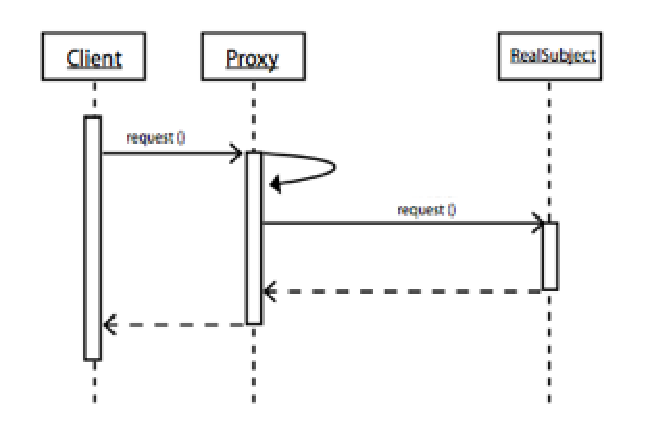
\includegraphics{ProxyIntegration}
\caption{Proxy Integration}
\label{fig:proxyintgr}
\end{figure}


To illustrate the use of MakeATest, an annotation was developed to verify the existence of a file. It is a simple example to demonstrate how to verify the existence of a local file, but could easily be modified to validate the existence of a remote file. \\


\begin{verbatim}
@MakeATestConfig(klass = 
      FileExistsExecute.class)
@Target({METHOD})
@Retention(RetentionPolicy.RUNTIME)
public @interface FileExists {
  String filePath();
}
\end{verbatim}
Figure 2. Annotation @FileExists.\\

Figure 4 shows how you want to use the annotations of MakeATest in our tests. We want to create two annotations @FileExists checks that after running the test if the file was actually created and the other annotation @FileNotExists verify that after running the test if the file was removed. \\
These annotations are created along with the classes of tests, since it has to be visible for both classes tests and also other classes of MakeATest. \\
An annotation is used to help to perform some predefined task. For the annotation "FileExists", the task is to verify that the specified file exists in the annotation system. \\
Figure 2 is the code for the annotation "FileExists", which follows the standard structure of the proposed annotation. Was included in the annotation MakeATest called "@MakeATestConfig. It is for this annotation that the framework knows the class responsible for executing the annotation that this will actually verify the existence of the file. The task of verifying the file is implemented in class "FileExistsExecute" that is described in property "klass" as show. \\
Figure 3 is the implementation of the execution class regarding the annotation "@FileExists". This execution class of the annotation, implements the methods defined in the interface MakeATestExecuteInterface as proposed. \\

\begin{verbatim}
public class FileExistsExecute implements 
        MakeATestExecuteInterface {
  @Override
  public void execute(
        Annotation annotation, 
        Method method, Object object) 
        throws FileNotFoundException {
    FileExists fileExists = 
        (FileExists) annotation;
    String path = fileExists.filePath();
    File f = new File(path);
    if (!f.exists()) {
      throw new FileNotFoundException();
    }
  }
  @Override
  public void execute(
        Annotation annotation, 
        Field field, Object object) 
        throws Exception {
  ...
  }
}
\end{verbatim}

Figure 3. Implementation of class execution annotation @FileExists.\\

\begin{verbatim}
@RunWith(MakeATestRunner.class)
public class FileCreationTest {
  @Test
  @FileExists(filePath="./file.txt")
  public void createFile() {
  ...
  }
  @Test
  @FileNotExists(filePath="./file.txt")
  public void deleteFile() {
  ...
  }
}
\end{verbatim}
Figure 4. Class test util the MakeATest.\\
When creating the body of the tests in Figure 4, we can call a feature of the software (downloaded from a remote file for example) that has as a result a creation of the file locally. When you run this TestCase, we have the annotation @FileExists processed and your class validation performed, verifying if the file exists or not, sending exception when necessary. \\
Because JUnit is already integrated with various IDEs, the eclipse could recognize the signs of success or failure in the test. \\



%\hfill mds 
%\hfill January 11, 2007
%\subsection{Subsection Heading Here}
%Subsection text here.

%\subsubsection{Subsubsection Heading Here}
%Subsubsection text here.


% An example of a floating figure using the graphicx package.
% Note that \label must occur AFTER (or within) \caption.
% For figures, \caption should occur after the \includegraphics.
% Note that IEEEtran v1.7 and later has special internal code that
% is designed to preserve the operation of \label within \caption
% even when the captionsoff option is in effect. However, because
% of issues like this, it may be the safest practice to put all your
% \label just after \caption rather than within \caption{}.
%
% Reminder: the "draftcls" or "draftclsnofoot", not "draft", class
% option should be used if it is desired that the figures are to be
% displayed while in draft mode.
%
%\begin{figure}[!t]
%\centering
%\includegraphics[width=2.5in]{myfigure}
% where an .eps filename suffix will be assumed under latex, 
% and a .pdf suffix will be assumed for pdflatex; or what has been declared
% via \DeclareGraphicsExtensions.
%\caption{Simulation Results}
%\label{fig_sim}
%\end{figure}

% Note that IEEE typically puts floats only at the top, even when this
% results in a large percentage of a column being occupied by floats.


% An example of a double column floating figure using two subfigures.
% (The subfig.sty package must be loaded for this to work.)
% The subfigure \label commands are set within each subfloat command, the
% \label for the overall figure must come after \caption.
% \hfil must be used as a separator to get equal spacing.
% The subfigure.sty package works much the same way, except \subfigure is
% used instead of \subfloat.
%
%\begin{figure*}[!t]
%\centerline{\subfloat[Case I]\includegraphics[width=2.5in]{subfigcase1}%
%\label{fig_first_case}}
%\hfil
%\subfloat[Case II]{\includegraphics[width=2.5in]{subfigcase2}%
%\label{fig_second_case}}}
%\caption{Simulation results}
%\label{fig_sim}
%\end{figure*}
%
% Note that often IEEE papers with subfigures do not employ subfigure
% captions (using the optional argument to \subfloat), but instead will
% reference/describe all of them (a), (b), etc., within the main caption.


% An example of a floating table. Note that, for IEEE style tables, the 
% \caption command should come BEFORE the table. Table text will default to
% \footnotesize as IEEE normally uses this smaller font for tables.
% The \label must come after \caption as always.
%
%\begin{table}[!t]
%% increase table row spacing, adjust to taste
%\renewcommand{\arraystretch}{1.3}
% if using array.sty, it might be a good idea to tweak the value of
% \extrarowheight as needed to properly center the text within the cells
%\caption{An Example of a Table}
%\label{table_example}
%\centering
%% Some packages, such as MDW tools, offer better commands for making tables
%% than the plain LaTeX2e tabular which is used here.
%\begin{tabular}{|c||c|}
%\hline
%One & Two\\
%\hline
%Three & Four\\
%\hline
%\end{tabular}
%\end{table}


% Note that IEEE does not put floats in the very first column - or typically
% anywhere on the first page for that matter. Also, in-text middle ("here")
% positioning is not used. Most IEEE journals/conferences use top floats
% exclusively. Note that, LaTeX2e, unlike IEEE journals/conferences, places
% footnotes above bottom floats. This can be corrected via the \fnbelowfloat
% command of the stfloats package.

\section{Conclusion}
A contribution of this work is the ease in creating annotations to verify the external effects caused by unit tests. \\
This feature occurs because the proposed solution is to create a framework that enable that the creation of the annotation and association with the implementation class can be done transparently to the developer. So the only developer's work is to implement the verification logic. \\
Another contribution is the aspect of reuse. How to check external effects could be repeated in methods, classes and even different applications, the annotations and implementing classes can be packaged in a jar and reuse in any project, since the annotations developed can be reused. \\
As future works we want to develop a study case using web services to verify the external effects. Integrations with frameworks like Mockito and Selenium are in our plans too. \\

% conference papers do not normally have an appendix


% use section* for acknowledgement
\section*{Acknowledgment}
The authors wish to express special thanks to friends and family for understanding the time dedicated to studies and for always being by our side.

% trigger a \newpage just before the given reference
% number - used to balance the columns on the last page
% adjust value as needed - may need to be readjusted if
% the document is modified later
%\IEEEtriggeratref{8}
% The "triggered" command can be changed if desired:
%\IEEEtriggercmd{\enlargethispage{-5in}}

% references section

% can use a bibliography generated by BibTeX as a .bbl file
% BibTeX documentation can be easily obtained at:
% http://www.ctan.org/tex-archive/biblio/bibtex/contrib/doc/
% The IEEEtran BibTeX style support page is at:
% http://www.michaelshell.org/tex/ieeetran/bibtex/
%\bibliographystyle{IEEEtran}
% argument is your BibTeX string definitions and bibliography database(s)
%\bibliography{IEEEabrv,../bib/paper}
%
% <OR> manually copy in the resultant .bbl file
% set second argument of \begin to the number of references
% (used to reserve space for the reference number labels box)
\begin{thebibliography}{1}

%\bibitem{IEEEhowto:kopka}
%H.~Kopka and P.~W. Daly, \emph{A Guide to \LaTeX}, 3rd~ed.\hskip 1em plus
% 0.5em minus 0.4em\relax Harlow, England: Addison-Wesley, 1999.


\bibitem{APACHE-SYNAPSE}
�Apache Synapse�. Available at http://synapse.apache.org/, 2010.

\bibitem{GOF}
Gamma, Erich et al , "Padr�es de projeto: Solu��es Reutiliz�veis de Software Orientado a Objetos", Bookman, 2000

\bibitem{GUERRA-PATTERN}
Guerra, Eduardo; Souza, Jerffeson; Fernandes, Clovis, "A Pattern Language for Metadata-based Frameworks", 16th Conference on Pattern Languages of Programming, Chicago, August, 2009.

\bibitem{GUERRA-2006}
Guerra, Eduardo, "Reflex�o + Anota��es - Uma Combina��o Explosiva", Revista Mundo Java,Ed. 0019, p.15-26, 2006.

\bibitem{GUERRA-2008}
Guerra, Eduardo, "Proxys Est�ticos e Din�micos", Revista Mundo Java, Ed. 0032, p. 51-56, 2008.

\bibitem{JUNIT}
�JUnit�. Available at http://junit.org/, 2010.


\end{thebibliography}

% that's all folks
\end{document}


